
\documentclass[aps,prl,reprint]{revtex4-2}
\usepackage{gensymb}
\usepackage{graphicx}
\usepackage{amsmath}
\usepackage{hyperref}
\usepackage{dsfont}
\usepackage{relsize}
\usepackage{wrapfig}
\usepackage{graphicx}
\usepackage{hyperref}
\hypersetup{colorlinks=true, citecolor=blue, urlcolor=blue, linkcolor=blue}


\begin{document}

% Use the \preprint command to place your local institutional report
% number in the upper righthand corner of the title page in preprint mode.
% Multiple \preprint commands are allowed.
% Use the 'preprintnumbers' class option to override journal defaults
% to display numbers if necessary
%\preprint{}

%Title of paper
\title{RUBY}

% repeat the \author .. \affiliation  etc. as needed
% \email, \thanks, \homepage, \altaffiliation all apply to the current
% author. Explanatory text should go in the []'s, actual e-mail
% address or url should go in the {}'s for \email and \homepage.
% Please use the appropriate macro foreach each type of information

% \affiliation command applies to all authors since the last
% \affiliation command. The \affiliation command should follow the
% other information
% \affiliation can be followed by \email, \homepage, \thanks as well.
\author{Trevor Smith, Alex Storrer}
\email[]{smith.tr@northeastern.edu}
\homepage[]{https://github.com/trevorm4x/}
%\thanks{}
%\altaffiliation{}
\affiliation{Northeastern University}


\date{\today}

\begin{abstract}
	Nothing is here
\end{abstract}


\maketitle

% body of paper here - Use proper section commands
% References should be done using the \cite, \ref, and \label commands
\section{Introduction}
% The Introduction should contain 1 or 2 paragraphs.
% Briefly state the physics underlying the experiment
% (what is being tested and why).
In the first phase of this experiment, we will analyze the room lighting, background 
lighting, and calibrate the spcectrometer. The calibration will be done by comparing
the measured wavelength of a green laser diode to its expected wavelength of 532 nm. 
We will then block out the background light with a black cloth, and
measure the transmission and absorption spectrum of our ruby crystal sample
by measuring the intensity of a wide spectrum white light and dividing by the 
intensity of the white light after it passes through the ruby. \\

In the next phase we will investigate ruby fluorescence. Ruby fluorescence is 
key in its ability to function as a laser, where, after being excited by an incident
light source, the electrons will quickly enter a meta-stable state from which they will
more slowly exit, emitting a photon. In this lab we will be observing the wavelength of
this emittance, which corresponds to the difference in energy levels, and the lifetime
of this meta-stable state. The latter will be measured by exciting the ruby with the
same laser, but powered by a function generator in a square wave pattern. The output
of the ruby will then be collected with a photodiode and measured on an oscilloscope. 


\section{Apparatus}
% List equipment components (manufacturer, model
% numbers and brief specifications). 

The apparatus consisted of the following.
\begin{itemize}
	\item Aluminum optical breadboard with 1/4-20 tapped holes
	\item Green laser diode
	\item Spectrometer, Ocean Optics USB4000FL, OceanView software, USB cable
	\item Lens, 200mm focal length
	\item Lens, 25mm focal length
	\item Mirror in adjustable x-y mount with rotational micrometer
	\item Photodiode (PD) detector
	\item Neutral-Density (ND) optical filter
	\item Long-Pass optical filter
	\item Optical Fibers, 50 and 600 micron core
	\item Black cloth
	\item White light illuminator
	\item Ruby Crystal, Al$_2$O$_3$:Cr, approximately 0.05\% Cr
	\item Oscilloscope, Tektronix TDS1052B
	\item Signal Generator, GW Instek GFG-8216A
	\item BNC Cables and T adapter
\end{itemize}

\section{Room Light Spectrum and Calibration}

\subsection{Procedure}
% Briefly describe the experimental procedures (in your own words, but don’t overdo it)
% Discuss calibrations, etc., if required
% Include necessary equations and put them on their own line (number them, e.g. “Eq. (3)”)
% Include plots showing relevant results (label each figure, e.g. “Fig. 3”, with caption).
% Describe what you found (describe what the plot illustrates)

First, a baseline for background noise in measurements made pointed at the breadboard
was established. The OceanView software was used to tune the Scans to Average setting,
which controls the amount of time the spectrometer collects incoming photons,
to maximize the usage of the input bits of that device. This step would be performed
for each spectrometer measurement. \\

Next, the spectrometer was calibrated using the 532 nm green laser, because the
basic function of the laser will remain unchanged from its factory settings due to
the nature of how laser light is produced, while a spectrometer as a measurement
device relies on mirrors which can likely change their adjustment over time. The laser
was connected directly to the fiber-optic cable, and then to the spectrometer, which
removed any effect of the background noise.\\

Finally, the fiber-optic cable was pointed directly at the lab lights to analyze the 
spectral signature of the fluorescent lighting and other lightsources.\\

\subsection{Results}


The background measurements shown in fig. \ref{bkg} were found not to be useful, as 
the two other measurements made without the black cloth covering would be 
substantially brighter than the background noise, and the black cloth would be used 
for all future, more carefully controlled tests. This measurement may still be
relevant if any of the peaks sneak into any of the the other data they shouldn't be 
in.\\

\begin{figure}[h]
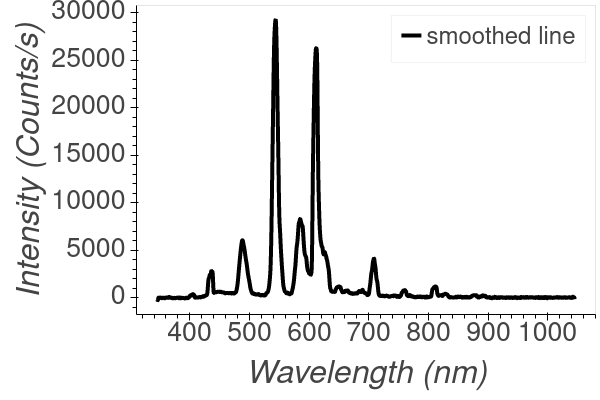
\includegraphics[width=0.4\textwidth]{../Images/l3_A_bkg.png}
\caption{\label{bkg}}
\end{figure}

The spectrometer measurement of the green laser was indeed found to be just over 533 nm,
meaning that all wavelength measurements using the spectrometer must be adjusted by 
1 nm. This was done proactively when loading the data from .txt file for the rest of the
lab involving the spectrometer, so all reported graphs and numbers have been corrected 
by this constant amount of 1.094 nm.

\begin{figure}[h]
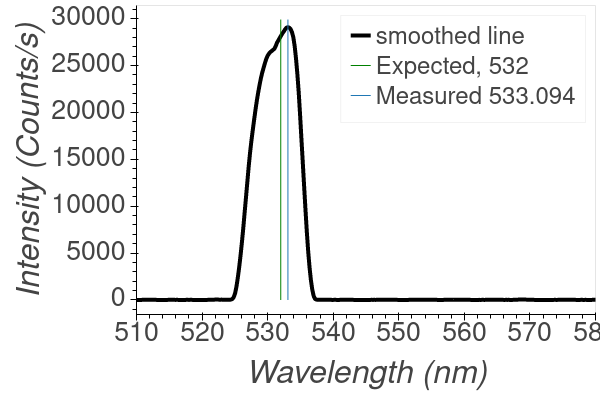
\includegraphics[width=0.4\textwidth]{../Images/l3_A_green.png}
\caption{\label{green}}
\end{figure}

Finally the lab light spectrum was analyzed, and is given in fig.\ref{lablight}.
The 6 largest peaks were found, and their
characteristic linewidth calculated. The narrowest one was at 435.3 nm, which 
corresponds to a violet color, with a linewidth of 1.9 nm. \\

It is interesting to briefly explore why there are separate peaks. Flourescent lights
are percieved as white, but the white light source used later in the lab will have
a significantly different spectral signature in spite of being percieved in much
the same way. This is due to the nature of the photo-receptors in our eyes. The three
color-receptors in fact overlap in the wavelengths they percieve, and the brain 
compensates for these overlaps by just adding them together. This adding together of
percieved light is why, as we see in the table \ref{widths}, orange + green + yellow + 
violet + red light = white light to our eyes. Flourescent bulbs create the illusion
of white light by producing just a few different color lights, with a few different
materials. \\

\begin{figure}[h]
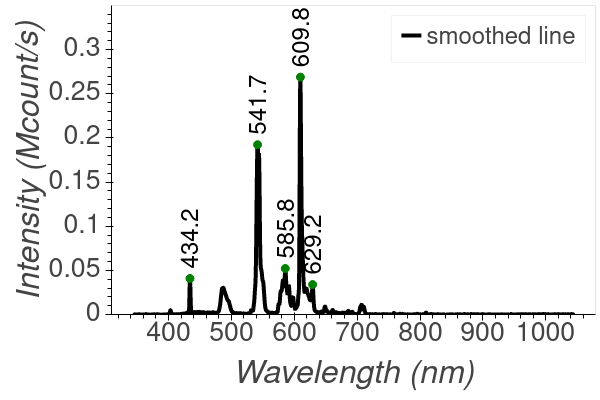
\includegraphics[width=0.4\textwidth]{../Images/l3_A_lablight.png}
\caption{\label{lablight}}
\end{figure}


\begin{table}[h]
\begin{tabular}{lrrl}
\toprule
Wavelength (nm) &  Intensity (cps) &  Linewidth (nm) &   Color \\
\hline
609.8 &     268854 &    3.3 &  Orange \\
541.7 &     192323 &    6.7 &   Green \\
585.8 &      52107 &    8.3 &  Yellow \\
434.2 &      40834 &    1.9 &  Violet \\
629.2 &      33929 &    2.2 &     Red \\\hline
\hline
\end{tabular}
\label{widths}
\end{table}

\section{Absorption Spectrum}

\subsection{Procedure}
In this phase of the lab the absorption spectrum of the ruby sample is measured. Here
we will use a white light source with a smooth output spectrum, and compare the
spectral signature of white light that does not pass through the ruby and white light
that does. The white light source was placed about 10 cm away from the FO cable 
connected to the spectrometer, and the ruby was mounted between them on a swivel to 
easily move in and out of the way of the beam. After everything was secured and aligned,
the black cloth was placed over the measurement setup to block out background noise. 
A measurement was made with and without the ruby crystal in the beam's path.
Measurements on the spectrogram were calibrated to optimize the use of its measurement
range, and the wavelengths measured were corrected by the above specified amount.


\subsection{Results}
The background noise was subtracted from each spectrum, and both are plotted in fig. \ref{ruby-no-ruby}.

\begin{figure}[h]
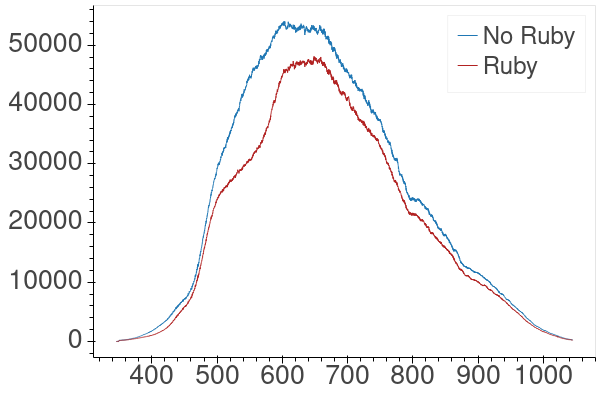
\includegraphics[width=0.4\textwidth]{../Images/l3_B_a.png}
\caption{\label{ruby-no-ruby}}
\end{figure}

Eq. \ref{alpha} was used to calculate various facets of the expected and measured
spectral signature of the ruby. First, we examine the expected transmission at
wavelength 700 nm, assuing that $\alpha$ = 0 and using the accepted value for n, 1.7.
The exponent evaluates to 1, and thus we get $(1-R)^2$ = 0.870. This value 
corresponds to the baseline (or maybe ceiling line) for how high transmission can
be at any wavelength regardless of absorption at that wavelength, due to the portion
of the signal that will be reflected due to the mismatch in n. \\

\begin{equation}
	\mathlarger{I = I_0(1-R)^2e^{-\alpha L}}
    \label{alpha}
\end{equation}

\begin{figure}[h]
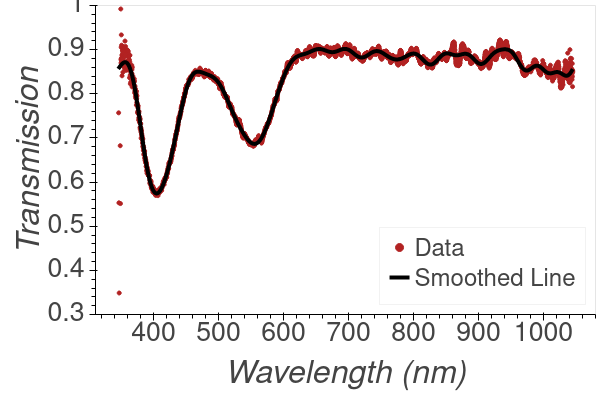
\includegraphics[width=0.4\textwidth]{../Images/l3_B_b.png}
\caption{\label{transmission_plot}}
\end{figure}

The transmission spectrum, given by eq. \ref{transmission}, was computed and plotted in
\ref{transmission_plot}.

\begin{equation}
	\mathlarger{T(\lambda) = I(\lambda)/I_0(\lambda)}
    \label{transmission}
\end{equation}

The spectrum of the absorption coefficient as a function of wavelength, 
$\alpha(\lambda)$ was computed via eq. \ref{alpha2}, which was derived from eq. 
\ref{alpha}, and plotted in fig. \ref{absorption}.

\begin{equation}
	\mathlarger{\alpha = \frac{-1}{L} \cdot ln\left(\frac{T}{(1-R)^2}\right)}
	\citation{\label{alpha2}, derived from \ref{alpha}}
\end{equation}

\begin{figure}[h]
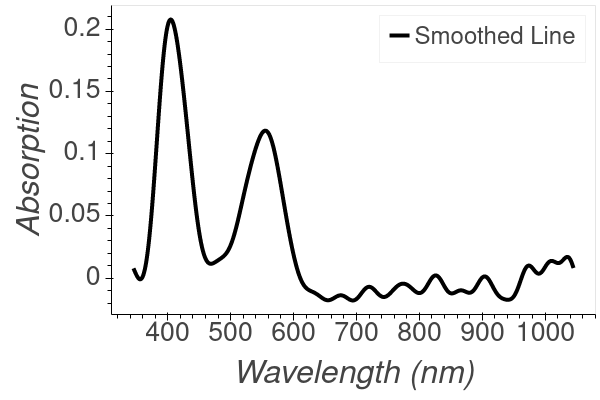
\includegraphics[width=0.4\textwidth]{../Images/l3_B_c.png}
\caption{\label{absorption}}
\end{figure}

The absorption peaks are centered at 400 and 550 nm, which correspond to the wavelengths
of light that the ruby absorbs. These correspond to, essentially, the other colors 
that aren't red, showing that the ruby appears red due to the red light passing through
it. The wavelength, widths and absorption lengths are given in table \ref{abs}. The
uncertainty displayed in the table was found by averaging the difference between the
raw, noisy data, and the smoothed line (smoothed using a simple lowpass filter in the
frequency domain).

\begin{table}[h]
\begin{tabular}{lrrll}
\toprule
Peak &  Wavelength (nm) &  Width (nm) &          alpha ($m^{-1}$) &        1/alpha (m) \\
\hline
1 &              404 &        56.0 &  0.206+/-0.005 &  4.9 +/- 0.1   \\
2 &              552 &        66.5 &  0.118+/-0.005 &  8.4 +/- 0.4   \\
\hline
\hline
\end{tabular}
\caption{\label{abs}}
\end{table}

\newpage
\subsection{Conclusions}

\section{Summary}


\begin{widetext}
\begin{center}
\begin{table}[h]
\renewcommand{\arraystretch}{1.35}
\setlength{\tabcolsep}{10pt}
\caption{\label{}Measured and accepted values of the speed of light and refractive index of various materials.}
\begin{tabular}{|c|c|c|c|c|}
%\hline
\toprule
Apparatus &  $\eta$ (\%) & Accepted $\eta$ value & Refs. & Deviation \\
\colrule
Photovoltaic Cell &  $15 \pm 2$ & $17 \pm 2.5$ & \cite{Solar Cell} & $0\sigma$  \\
\colrule
Elecrolyzer &  $87 \pm 6$ & 80 & \cite{Electrolyzer} & $2\sigma$  \\
\colrule
Hydrogen Fuel Cell &  $49 \pm 5$ & 60 & \cite{Fuel Cell} & $-3\sigma$  \\
%\hline
\botrule
\end{tabular}
\end{table}
\end{center}
\end{widetext}





\begin{thebibliography}{9}
%
\bibitem{HHV} 
Wikipedia, Heat of Combustion: \\
\href{https://en.wikipedia.org/wiki/Heat_of_combustion}{https://www.wikepedia.com}
%
\bibitem{Solar Cell} 
Energysage, Most Efficient Solar Panels\\
\href{https://news.energysage.com/what-are-the-most-efficient-solar-panels-on-the-market/#:~:text=How%20efficient%20are%20solar%20panels,are%20not%20above%2020%25%20efficiency.}{https://www.energysage.com/}
%
\bibitem{Electrolyzer} 
Carbon Commentary, Hydrogen made by Electolysis\\
\href{https://www.carboncommentary.com/blog/2017/7/5/hydrogen-made-by-the-electrolysis-of-water-is-now-cost-competitive-and-gives-us-another-building-block-for-the-low-carbon-economy}{https://www.carboncommentary.com}
%

%
\bibitem{Fuel Cell} 
Energy.gov, Fuel Cell Fact Sheet\\
\href{https://www.energy.gov/sites/prod/files/2015/11/f27/fcto_fuel_cells_fact_sheet.pdf}{https://www.energy.gov}

\end{thebibliography}


\end{document}
%
% ****** End of file apstemplate.tex ******

